\section{Co-speech Gesture Inference}
\label{sec:co-speech_gesture_inference}
When given a speech as input, our system segments it into normalized feature blocks $\{\vect{A}_i^{\eqword{low}}, \vect{A}_i^{\eqword{high}}, \vect{T}_i, \vect{I}\}$ and then generates motion blocks $\{\vect{M}_i^*\}$ recursively, where 
\begin{align}
    \vect{M}_i^* = \mathcal{G}\left(
        \mathcal{E}_M\left(\vect{M}_{i-1}^*\right), 
        \mathcal{E}_A\left(\vect{A}^{\eqword{low}}_{i-1}, \vect{A}^{\eqword{low}}_{i}, \vect{A}^{\eqword{low}}_{i+1}\right), 
        \vect{s}_i^*, \vect{z}_i^*, \vect{P}
        \right),
    \label{eqn:gesture_inference}
\end{align}
and $\mathcal{G}, \mathcal{E}_M, \mathcal{E}_A$ are the components of the learned gesture generator. The generated motion blocks are then denormalized to their original length in the input speech, producing a realistic co-speech gesture animation. Note that we again use the asterisk~($*$) to indicate a computed quantity that is not provided directly in the speech. 

All the variables in \eqn\eqref{eqn:gesture_inference} are known except the gesture lexeme $\vect{s}^*$ and style code $\vect{z}^*$. As shown in \fig\ref{fig:system_overview}, our system learns two interpreters to compute them: the \emph{lexeme interpreter} $\mathcal{P}_s$ translates high-level speech features into the gesture lexemes $\vect{s}^*$, and the \emph{style interpreter} $\mathcal{P}_z$ predicts the style code $\vect{z}^*$ according to the low-level speech features. 

\begin{figure}[t]
    \centering
    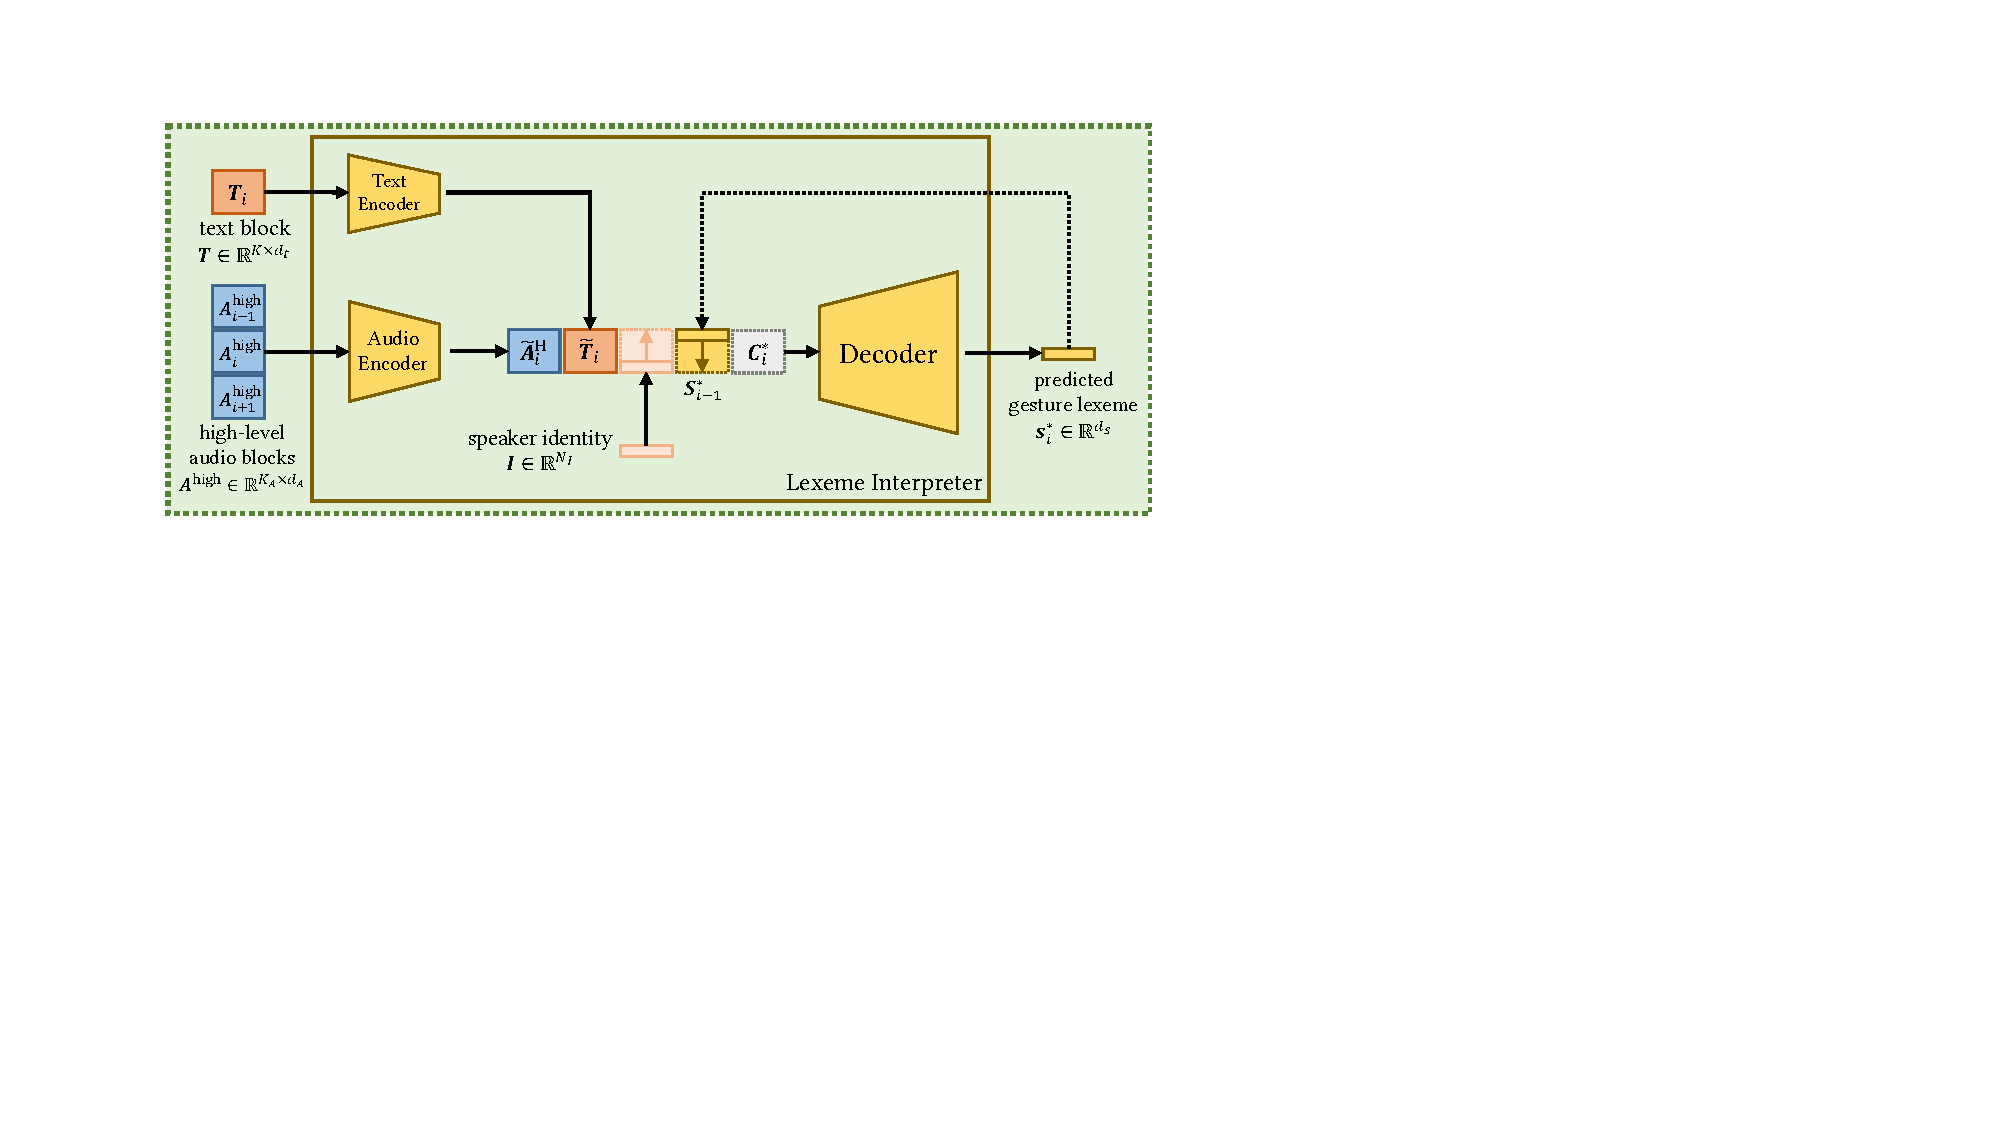
\includegraphics[width=\linewidth]{figures/fig5.pdf}
    \caption{Architecture of the lexeme interpreter.}
    \Description{}
    \label{fig:interpreters}
\end{figure}

\subsection{Lexeme Interpreter}
\label{subsec:lexeme_interpreter}
As illustrated in \fig\ref{fig:interpreters}, the lexeme interpreter is formulated as
\begin{equation}
    \vect{s}_i^*=\mathcal{P}_s(\vect{s}_{i-1}^*, \tildevect{A}_i^{\eqword{H}}, \tildevect{T}_i, \vect{I}), 
    \label{eqn:lex_interpreter}
\end{equation}
which is conditioned on the gesture lexeme of the last motion block $\vect{s}_{i-1}^*$, and the high-level features of the current speech block. Like the generator, the high-level audio features $\tildevect{A}_i^{\eqword{H}}\in\mathbb{R}^{K\times{}d_{\tilde{A}}}$ are computed using three consecutive audio blocks
\begin{equation}
    \tildevect{A}_i^{\eqword{H}}=\mathcal{E}_A^{\eqword{lex}}(\vect{A}^{\eqword{high}}_{i-1},\vect{A}^{\eqword{high}}_{i},\vect{A}^{\eqword{high}}_{i+1}),
\end{equation}
where each $\vect{A}^{\eqword{high}}$ contains the high-level representation of the input speech audio, and the encoder $\mathcal{E}_A^{\eqword{H}}$ is a single-layer fully connected network. 
%
The text feature $\tildevect{T}_i\in\mathbb{R}^{K\times{}d_{\tilde{t}}}$ is also extracted from the text representation of the speech block as 
\begin{equation}
    \tildevect{T}_i=\mathcal{E}_T^{\eqword{lex}}(\vect{T}_i),
\end{equation}
where $\mathcal{E}_T^{\eqword{lex}}$ is again a single-layer network. % that changes the dimensionality of the text representation $\vect{T}_i$. 
%
Lastly, the one-hot representation of the speaker ID, $\vect{I}$, is repeated $K$ times and converted into a feature block.

Those feature blocks can then be concatenated together and fed to an LSTM-based decoder to predict the next gesture lexeme $\vect{s}_i^*$. However, considering that the lexemes are selected from the discrete gesture lexicon, we can convert this regression problem into a classification problem. Specifically, instead of directly evaluating \eqn\eqref{eqn:lex_interpreter}, we can let $\mathcal{P}_s$ predict the probability that $\vect{s}_i^*$ is a specific lexeme in the gesture lexicon, then the lexeme with the maximum likelihood will be considered as the result.

\subsection{Style Interpreter}
The style interpreter shares a similar structure with the lexeme interpreter. It computes $\vect{z}_{i}^*$ as
\begin{equation}
    {\vect{z}}_{i}^{*} = \mathcal{P}_z\left(
        \vect{z}_{i-1}^*,
        \vect{s}_{i}^*,
        \mathcal{E}_T^{\eqword{style}}\left(\vect{T}_i\right), 
        \mathcal{E}_A^{\eqword{style}}\left(\vect{A}^{\eqword{low}}_{i-1},\vect{A}^{\eqword{low}}_{i},\vect{A}^{\eqword{low}}_{i+1}\right)
        \right),
    \label{eqn:style_interpreter}
\end{equation}
which is conditioned on the last style code and the new gesture lexeme computed by the lexeme interpreter. The low-level audio representation $\vect{A}^{\eqword{low}}$ is used in the style interpreter.

\subsection{Audio-Only Inference}
\label{subsec:inference_based_on_audio_only}
Both the two interpreters can be reformulated to take only the speech audio as input, where the features related to the text representation $\vect{T}$, and optionally the speaker ID $\vect{I}$, will be removed from \eqn\eqref{eqn:lex_interpreter} and \eqref{eqn:style_interpreter}.

In practice, these audio-only interpreters allow cross-language gesture generation, where the speech audio in another language can be taken as input to synthesize realistic gestures without further training. For example, we can utilize a pre-trained model on an English dataset to generate gestures that accompany a Chinese speech. We will show related experiments in Section \ref{subsec:evaluation}.

\subsection{Training}
During the training of the generator, we have computed the gesture lexeme $\vect{s}_i$ and the style code $\vect{z}_i$ of every motion block in the training dataset. We then train the two interpreters using these results as the ground truth. We minimize the standard categorical cross-entropy loss to train the lexeme interpreter, while the MSE loss is used for the style interpreter.

\subsubsection{Silent Period Hint}
A speaker typically stops gesticulating during a silent pause \cite{graziano2018silence}. Such behaviors are often crucial to the naturalness of a co-speech gesture animation. However, we find that it is often difficult for a gesture generator to deal with silent periods well, even in recent successful systems such as \cite{alexanderson2020style,kucherenko2020gesticulator}. The speech-gesture datasets may lack necessary motion, and some specific generator models, such as LSTM, may exhibit generative inertia that makes it difficult to become stationary in time.

To solve this problem, we develop a new approach, which we refer to as the \emph{silent period hint}, to encourage the lexeme interpreter to compute a specific \emph{silent lexeme} that corresponds to a silent gesture when encountering a silent period. 
We check all the lexemes in the lexicon and label a number of stationary ones as the silent lexemes. Notably, the silent lexemes can be automatically labeled by finding such a lexeme corresponding to an empty text word. Then, when a training audio block is in a silent period, which can be detected by the data module of our system, we will force the lexeme interpreter to output the silent lexeme that is the nearest to the current lexeme in the latent space.
Moreover, a silent data augmentation is applied when training the generator. We find data blocks that contain empty words and randomly insert $0\sim{}10$ consecutive silent blocks after them. The silent block above includes four different features: (a) the audio feature is the environmental noise; (b) the style code is set to zero; (c) the gesture lexeme is the silent lexeme that is the nearest to the previous lexeme in the latent space; and (d) the motion is a stationary pose that is the same as the last frame of the previous motion block. In total, the amount of the inserted silent blocks accounts for $5\%$ of the whole training set.